\usepackage[T1]{fontenc}
\usepackage[latin1]{inputenc}

\usepackage{amsmath}
\usepackage{amsfonts}
\usepackage{amssymb}
\usepackage{wrapfig}
\usepackage{tikz}
\usetikzlibrary{arrows,shapes,backgrounds,mindmap}
\usepackage{verbatim}
\usepackage{graphics}
\usepackage{multimedia} 
\usepackage{multicol}
\usepackage{ifthen}
\usepackage{cases}
\usepackage{tabularx}
%\usepackage{biblatex}
%\usepackage{natbib}
\usepackage{multimedia}

% For every picture that defines or uses external nodes, you'll have to
% apply the 'remember picture' style. To avoid some typing, we'll apply
% the style to all pictures.
\tikzset{
    branch color/.style={
        concept color=#1!white,
        every child/.append style={concept color=#1!white!30!white},
    },
    level width/.store in=\tikzlevelwidth,
    level height/.store in=\tikzlevelheight
}
\tikzstyle{every picture}+=[remember picture]

% By default all math in TikZ nodes are set in inline mode. Change this to
% displaystyle so that we don't get small fractions.
\everymath{\displaystyle}

%\bibpunct{[}{]}{;}{s}{,}{,}
%\renewcommand{\cite}{\citep}
\def\newblock{\hskip .11em plus .33em minus .07em}

\usepackage[french, english]{babel}

\usepackage{accents}
\newcommand{\fallen}[1]{\accentset{\times}{#1}}

 \DeclareMathOperator\cov{cov}

\mode<presentation>
{
  \usetheme{Warsaw}
  % or ...

  \setbeamercovered{transparent}
  % or whatever (possibly just delete it)
}

\useoutertheme{mysmoothbars}
\useinnertheme{default}
\usefonttheme[onlymath]{serif}

\usetheme{Frankfurt}
\usepackage{remreset}
\makeatletter
\@removefromreset{subsection}{section}
\makeatother
\setcounter{subsection}{0}

\setbeamertemplate{itemize item}[square]
\setbeamertemplate{itemize subitem}[square]
\setbeamertemplate{itemize subsubitem}[square]
\setbeamertemplate{enumerate item}[default]
\setbeamertemplate{enumerate subitem}[default]
\setbeamertemplate{enumerate subsubitem}[default]
\usecolortheme{dove}
\setbeamertemplate{frametitle}[default][center]


\setbeamertemplate{section in toc}[sections numbered]
\setbeamertemplate{subsection in toc}[default]
\setbeamertemplate{bibliography item}[triangle]
\setbeamerfont{section in toc}{size=\scriptsize }
\setbeamerfont{subsection in toc}{size=\tiny }
\setbeamerfont{alerted text}{series=}
\setbeamerfont{bibliography item}{size=\tiny} 
\setbeamercolor{alerted text}{fg=red} 

%\pgfdeclareimage[height=96mm,width=128mm]{back}{img/background43-2}
%\setbeamertemplate{background}{\pgfuseimage{back}}
 % \setbeamersize{text margin right=2cm}
  
  
\geometry{ 
tmargin=0cm,    % Marge haute
bmargin=3cm,    % Marge basse
lmargin=0.5cm,    % Marge gauche
rmargin=0.5cm,    % Marge droite
headheight=0cm, % Entete
headsep=0cm,    % S�parateur entete
footskip=0cm    % Pied de page
}




\setbeamertemplate{navigation symbols}
{%
}
 

\newcommand{\linejump}{\[\therefore\]} 

\DeclareMathOperator{\Tr}{Tr}
\DeclareMathOperator{\rank}{rank}
\DeclareMathOperator{\modulo}{modulo}
\DeclareMathOperator{\E}{\mathbb E}
\DeclareMathOperator{\argmin}{argmin}
\DeclareMathOperator{\diag}{diag}

\newcommand{\ka }{{k:\alpha}}

\title[Motion Generation for Pulling a Fire Hose by a Humanoid Robot] % (optional, use only with long paper titles)
{\huge Motion Generation for Pulling a Fire Hose by a Humanoid Robot}


%resets the environment to a one with less lost space after the title
\let\oldframe\frame
\let\endoldframe\endframe
\renewenvironment{frame}[2][c]{\oldframe[#1]{#2} \vspace{-20pt}}{\endoldframe}

\newenvironment{cadre}{\begin{minipage}[c][\textheight][c]{\linewidth}}{\end{minipage}}


%gives access to the text height
\makeatletter\let\frametextheight\beamer@frametextheight\makeatother



\author 
{\textbf{Maximilien~Naveau (\texttt{mnaveau@laas.fr})}, %Olivier~Stasse(\texttt{ostasse@laas.fr})
}


\institute[] % (optional, but mostly needed)
{
Gepetto team - LAAS / CNRS - Toulouse, France\\

\includegraphics[height=2cm]{logo/LogoLAASCarnot.png}
\hspace{0.5cm}
\includegraphics[height=2cm]{logo/koroibot-logo}
\hspace{0.5cm}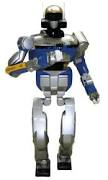
\includegraphics[height=2cm]{hrp2.jpeg}
\hspace{0.5cm}
\includegraphics[height=1cm]{logo/logoAIST.jpeg}\\
}
% - Use the \inst command only if there are several affiliations.
% - Keep it simple, no one is interested in your street address.

\date % (optional, should be abbreviation of conference name)
{JNRH - Toulouse - 2016}
% - Either use conference name or its abbreviation.
% - Not really informative to the audience, more for people (including
%   yourself) who are reading the slides online

\subject{Robotics}
% This is only inserted into the PDF information catalog. Can be left
% out. 


% If you have a file called "university-logo-filename.xxx", where xxx
% is a graphic format that can be processed by latex or pdflatex,
% resp., then you can add a logo as follows:

%\pgfdeclareimage[height=0.5cm]{university-logo}{logo/koroibot-logo}
%\logo{\pgfuseimage{university-logo}}



% Delete this, if you do not want the table of contents to pop up at
% the beginning of each subsection:
%\AtBeginSubsection[]
%{
%  \begin{frame}<beamer>{Outline}
%  \vskip-6ex
%   \tableofcontents[currentsection,currentsubsection]
% \end{frame}
%}

%\AtBeginSection[]
%{
%  \begin{frame}<beamer>{Outline}
%  \vskip-6ex
%      \tableofcontents[currentsection]
%  \end{frame}
%}

\newcommand{\sectionend}{
  \begin{frame}<beamer>{Outline}
    \vskip-6ex
    \tableofcontents[currentsection] 
  \end{frame}
}

\newcommand{\subsectionend}{
  \begin{frame}<beamer>{Outline}
    \vskip-6ex     
    \tableofcontents[currentsection,currentsubsection]
  \end{frame}
}


% If you wish to uncover everything in a step-wise fashion, uncomment
% the following command: 

%\beamerdefaultoverlayspecification{<+->}

\newcommand{\chwithnonumbers}{false}
\newcommand{\bq}{{\bf q}}
\newcommand{\bhq}{{\bf \hat{q}}}
\newcommand{\eq}[1]{(\ref{#1})}
\newcommand{\mbf}[1]{{\mathbf{#1}}}
\newcommand{\deriv}[1]{d#1}

\newcommand{\R}{{\mathbb{R}}}

\newcommand{\md}{d}

% --- Notation --- %
\newcommand{\mProjec}[1]{\mbf{Proj}(#1)}
\newcommand{\mP}[1]{\mbf{P_{#1}}}
\newcommand{\mPaug}[1]{\mbf{P_{#1}^{A}}}
\newcommand{\mProj}[2]{\mbf{P_{#1 \dots #2}}}

\newcommand{\mC}[1]{\mbf{C_{#1}}}

\newcommand{\mL}[1]{\mbf{L_{#1}}}
\newcommand{\mpL}[1]{\mbf{L_{#1}^{+}}}
\newcommand{\maL}[1]{\mbf{\widehat{L}_{#1}}}
\newcommand{\mapL}[1]{\mbf{\widehat{L_{#1}^{+}} }}
\newcommand{\mpaL}[1]{\mbf{\widehat{L}_{#1}^{+}}}
\newcommand{\mLaug}[1]{\mbf{L_{#1}^{A}}}
\newcommand{\mpLaug}[1]{\mbf{L_{#1}^{A+}}}
\newcommand{\mtL}[1]{\mbf{\widetilde{L_{#1}}}}
\newcommand{\mtpL}[1]{\mbf{\widetilde{L_{#1}}^{+}}}

\newcommand{\mJ}[1]{\mbf{J_{#1}}}
\newcommand{\mhJ}[1]{\mbf{\hat{J}_{#1}}}
\newcommand{\mdJ}[1]{\mbf{\dot{J}_{#1}}}
\newcommand{\mpJ}[1]{\mbf{J_{#1}^{+}}}
\newcommand{\maJ}[1]{\mbf{\widehat{J}_{#1}}}
\newcommand{\mapJ}[1]{\mbf{\widehat{J_{#1}^{+}} }}
\newcommand{\mpaJ}[1]{\mbf{\widehat{J}_{#1}^{+}}}
\newcommand{\mJaug}[1]{\mbf{J_{#1}^{A}}}
\newcommand{\mpJaug}[1]{\mbf{J_{#1}^{A+}}}
\newcommand{\mtJ}[1]{\mbf{\widetilde{J_{#1}}}}
\newcommand{\mtpJ}[1]{\mbf{\widetilde{J_{#1}}^{+}}}

\newcommand{\me}[1]{\mbf{e_{#1}}}
\newcommand{\mec}[1]{\mbf{e_{#1}^{*}}}
\newcommand{\medot}[1]{\mbf{\dot{e_{#1}}}}
\newcommand{\meddot}[1]{\mbf{\ddot{e_{#1}}}}
\newcommand{\mde}[1]{\mbf{\md e_{#1}}}

\newcommand{\mte}[1]{\mbf{\widetilde{e}_{#1}}}
\newcommand{\mtedot}[1]{\mbf{\widetilde{\dot{e}_{#1}}}}
\newcommand{\mteddot}[1]{\mbf{\widetilde{\ddot{e}_{#1}}}}

\newcommand{\medotc}[1]{\mbf{\dot{e_{#1}}^{*}}}
\newcommand{\meddotc}[1]{\mbf{\ddot{e_{#1}}^{*}}}

\newcommand{\ms}[1]{\mbf{s_{#1}}}
\newcommand{\msdot}[1]{\mbf{\dot{s_{#1}}}}
\newcommand{\msd}[1]{\mbf{s^{*}_{#1}}}

\newcommand{\mq}{\mbf{q}}
\newcommand{\mqdot}{\mbf{\dot{q}}}
\newcommand{\mqddot}{\mbf{\ddot{q}}}
\newcommand{\mdq}[1]{\mbf{\md q_{#1}}}
\newcommand{\mqr}{\mbf{\rho}}
\newcommand{\mqrlim}{\mbf{\rho}_{lim}}
\newcommand{\mqrdot}{\mbf{\dot{\rho}}}
\newcommand{\mQmax}[1]{\mbf{Q_{#1}}^{MAX}}
\newcommand{\mQmin}[1]{\mbf{Q_{#1}}^{MIN}}

\newcommand{\mr}{\mbf{r}}
\newcommand{\mrdot}{\mbf{\dot{r}}}
\newcommand{\mscrew}{\mbf{v}}

\newcommand{\mres}{\mbf{\rho}}

\newcommand{\mevit}{\mbf{g}^{JointLim}}

\newcommand{\mpot}[1]{V_{#1}}
\newcommand{\mFpot}[1]{\mbf{g}_{#1}}
\newcommand{\mf}[1]{\mbf{f}_{#1}}
\newcommand{\mg}{\mbf{g}}
\newcommand{\mgrad}[1]{{\nabla}_{#1}}
\newcommand{\mgradT}[1]{{\nabla}_{#1}^{\top}}

\newcommand{\qlim}[1]{\bar{q}_{#1}}
\newcommand{\qmin}[1]{\bar{q}^{\min}_{#1}}
\newcommand{\qmax}[1]{\bar{q}^{\max}_{#1}}
\newcommand{\qlmin}[1]{\bar{q}^{\min}_{\ell#1}}
\newcommand{\qlmax}[1]{\bar{q}^{\max}_{\ell#1}}

\newcommand{\mqlim}[1]{\qlim{#1}}
\newcommand{\mqmin}[1]{\qmin{#1}}
\newcommand{\mqmax}[1]{\qmax{#1}}
\newcommand{\mqlmin}[1]{\qlmin{#1}}
\newcommand{\mqlmax}[1]{\qlmax{#1}}


\newcommand{\mvv}{\hbox{\boldmath $v$}}
\newcommand{\mvomega}{\hbox{\boldmath $\omega$}}


\newcommand{\mI}{\mbf{I}}

\newcommand{\derive}[2]{\frac{\deriv{#1}}{\deriv{#2}}}
\newcommand{\dpartial}[2]{\frac{\partial{#1}}{\partial{#2}}}

\newcommand{\mdeuxD}{2-D }
\newcommand{\mtroisD}{3-D }
\newcommand{\mdeuxDd}{2-1/2-D }



\newcommand{\att}[1]{\underline{#1}}

% \newcommand{\argmax}[1]{\arg\!\max_{\!\!\!\!\!\!\!\!\!\!\!\!\!\!\!\!#1}}
\newcommand{\argmax}[1]{\mathop{\arg\!\max}_{#1}}
%\newcommand{\argmax}[1]{\mathop{\mbox{argmax}}_{#1}}
\newcommand{\mdint}{\int\!\!\!\int}


\newcommand{\mCam}{{\bf C}}
\newcommand{\mCamR}{{\bf \psi_c}}

\ifthenelse{\equal{\chwithnonumbers}{true}}{
\newcommand{\newchapter}{\chapter*}
\newcommand{\newsection}{\section*}
\newcommand{\newsubsection}{\subsection*}
}
{
\newcommand{\newchapter}{\chapter}
\newcommand{\newsection}{\section}
\newcommand{\newsubsection}{\subsection}
}

\newcommand{\pcrefc}{PC^{ref}_{c}}
\newcommand{\cpcrefc}{CPC^{ref}_{c}}
\newcommand*\rfrac[2]{{}^{#1}\!/_{#2}}






\newcommand{\I}{\mathbb{I}}

\newcommand{\NT}{\textup{N}}
\newcommand{\NX}{n_\textup{x}}
\newcommand{\NU}{n_\textup{u}}

\newcommand{\FL}{\textup{FL}}
\newcommand{\FR}{\textup{FR}}

\newcommand{\HL}{\textup{HL}}
\newcommand{\HR}{\textup{HR}}

\newcommand{\ini}{\textup{ini}}
\newcommand{\fin}{\textup{fin}}
\newcommand{\tini}{t_{\textup{ini}}}
\newcommand{\tfin}{t_{\textup{fin}}}

\newcommand{\Qf}{{\bf Q}_{i}}
\newcommand{\tauf}{\mathbf{\tau}_i}
\newcommand{\pf}{{\bf p}_{i}}
\newcommand{\ff}{{\bf f}_{i}}
\newcommand{\ffz}{f_{i,z}}
\newcommand{\ffx}{f_{i,x}}
\newcommand{\ffy}{f_{i,y}}
\newcommand{\com}{{\bf c}}
\newcommand{\dcom}{\dot{\bf c}}
\newcommand{\ddcom}{\ddot{\bf c}}
\newcommand{\dddcom}{\dddot{\bf c}}

\newcommand{\ffk}{{\bf f}^k_{i}}
\newcommand{\ffkx}{{\bf f}^k_{i,x}}
\newcommand{\ffky}{{\bf f}^k_{i,y}}
\newcommand{\ffkz}{{\bf f}^k_{i,z}}

\newcommand{\ffkl}{{\bf f}^{k+l}_{i}}
\newcommand{\ffklz}{{\bf f}^{k+l}_{i,z}}


% define matrix and vector commands
\newcommand  {\const}[1]{\mathrm{#1}}
\renewcommand{\vec}  [1]{\mathbf{#1}}
\newcommand  {\mat}  [1]{\mathrm{#1}}

\newcommand*{\Scale}[2][4]{\scalebox{#1}{$#2$}}%
\newcommand*{\Resize}[2]{\resizebox{#1}{!}{$#2$}}%

% Robot model
\newcommand{\robm}{\it model}

% Generalized inertia matrix
\newcommand{\im}{\bf H}

% Centrifugal and Coriolis matrix
\newcommand{\gbf}{\bf C}

% Generalized forces.
\newcommand{\mtau}{\bm \tau}

% Local variables
\newcommand{\mvJi}{{\bf v}_{Ji}}
\newcommand{\mcJi}{{\bf c}_{Ji}}

\newcommand{\BIN}{\begin{bmatrix}}
\newcommand{\BOUT}{\end{bmatrix}}
\newcommand{\am}{\mathcal{L}}
\newcommand{\lm}{\mathcal{K}}

%\includeonly{Section5}
\graphicspath{{./}{../}{../figures/}{../videos/}}


\usepackage{biblatex}
\bibliography{16-jnrh-mnaveau.bib}
\renewcommand{\footnotesize}{\scriptsize}
%
%\tikzset{every picture/.style={font issue=\footnotesize},
%         font issue/.style={execute at begin picture={#1\selectfont}}
%        }

% Show the table of contents at the beginning of every subsection.
\AtBeginSection[]{
    \vspace*{-1cm}
    \frametitle{Table of contents}
    \tableofcontents[current,currentsubsection]
}

